% ==============================================================================
% frontmatter/titlepage.tex — ปกใน Smart Agriculture & Soil-Plant AI Handbook
% ปกกราฟิกเวกเตอร์ต้นฉบับ ออกแบบสำหรับหนังสือขนาด 6 x 9 นิ้ว
% ==============================================================================
\begin{titlepage}
\thispagestyle{empty}
\centering
\begingroup
\pagecolor{black!94}
\color{white}

\vspace*{0.24in}

{\fontsize{9}{12}\selectfont\bfseries\color{green!45!yellow}
EMBEDDED AI \& EDGE AIoT \enspace / \enspace PRECISION AGRICULTURE}

\vspace{0.12in}
{\color{green!45!yellow}\rule{0.78in}{1.2pt}}

\vspace{0.14in}
{\fontsize{9.5}{13}\selectfont\bfseries\color{white!80}
คู่มือการจัดเตรียมชุดข้อมูลและการฝึกอบรม}

\vspace{0.04in}
{\fontsize{21}{26}\selectfont\bfseries
{\color[HTML]{FF9800}ปัญญาประดิษฐ์ฝังตัว}{\color{white!85}และ}{\color[HTML]{FF7043}เอดจ์}{\color[HTML]{4FC3F7}เอไอโอที}\\[-0.01in]
{\color[HTML]{81C784}เพื่อการเกษตร}{\color{white!85}และ}{\color[HTML]{4DD0E1}สิ่งแวดล้อม}}

\vspace{0.07in}
{\fontsize{8.5}{11}\selectfont\color{white!80}
(Embedded AI \& Edge AIoT for Agriculture and Environment:\\[2pt]
From Pixel-Level Bio-Vision \& Soil Sensing to Deployable Field Diagnostics)}

\vspace{0.13in}

% Original vector illustration: a sunlit, layered farm landscape with a
% friendly AI field sensor at its center.
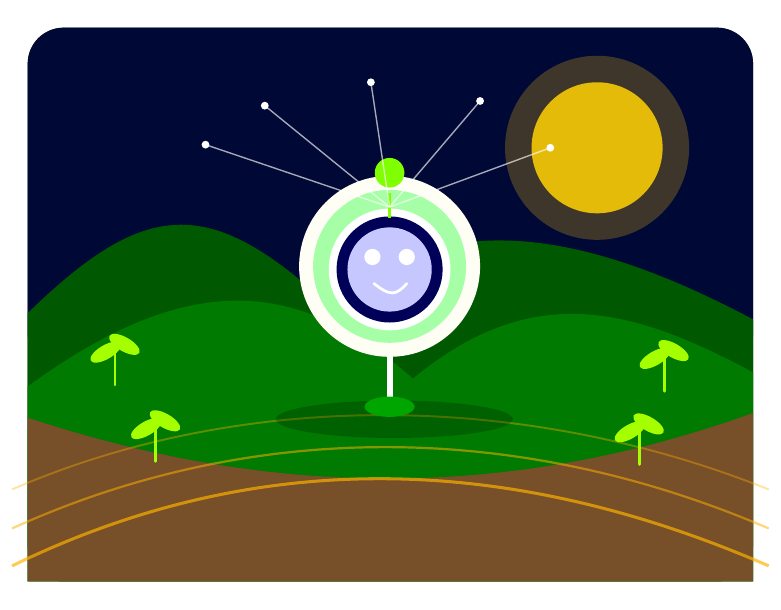
\begin{tikzpicture}[x=0.78in,y=0.78in]
  \useasboundingbox (0,0) rectangle (4.65,3.55);

  % Soft atmospheric sky
  \fill[rounded corners=13pt,green!12!black]
    (0,0) rectangle (4.65,3.55);
  \fill[rounded corners=13pt,blue!30!black,opacity=.72]
    (0,1.35) rectangle (4.65,3.55);
  \fill[yellow!70!orange,opacity=.88] (3.65,2.78) circle (.42);
  \fill[yellow!55!orange,opacity=.25] (3.65,2.78) circle (.59);

  % Distant hills
  \fill[green!35!black]
    (0,1.72) .. controls (.75,2.45) and (1.16,2.48) .. (1.92,1.78)
    .. controls (2.64,2.37) and (3.48,2.3) .. (4.65,1.68)
    -- (4.65,0) -- (0,0) -- cycle;
  \fill[green!48!black]
    (0,1.25) .. controls (1.03,2.00) and (1.73,1.95) .. (2.47,1.30)
    .. controls (3.23,1.93) and (3.87,1.76) .. (4.65,1.34)
    -- (4.65,0) -- (0,0) -- cycle;

  % Warm, curved crop rows
  \fill[brown!62!black]
    (0,0) -- (4.65,0) -- (4.65,1.08)
    .. controls (3.12,.53) and (1.6,.52) .. (0,1.05) -- cycle;
  \draw[orange!60!yellow,opacity=.68,line width=1.1pt]
    (-.1,.10) .. controls (1.40,.83) and (3.00,.86) .. (4.75,.10);
  \draw[orange!60!yellow,opacity=.52,line width=.8pt]
    (-.1,.34) .. controls (1.42,1.03) and (3.12,1.04) .. (4.75,.34);
  \draw[orange!60!yellow,opacity=.36,line width=.7pt]
    (-.1,.59) .. controls (1.35,1.22) and (3.15,1.23) .. (4.75,.59);

  % Oversized friendly field sensor
  \fill[black,opacity=.2] (2.35,1.04) ellipse (.76 and .12);
  \draw[white!70,line width=2.2pt,line cap=round] (2.32,1.13) -- (2.32,1.55);
  \fill[green!65!black] (2.32,1.12) ellipse (.16 and .065);
  \fill[white!96!yellow] (2.32,2.02) circle (.58);
  \fill[green!35!white] (2.32,2.02) circle (.49);
  \fill[white] (2.32,2.00) circle (.39);
  \fill[blue!35!black] (2.32,2.00) circle (.34);
  \fill[blue!22!white] (2.32,2.00) circle (.27);
  \fill[white] (2.21,2.08) circle (.052);
  \fill[white] (2.43,2.08) circle (.052);
  \draw[white,line width=1pt,line cap=round]
    (2.22,1.91) .. controls (2.32,1.83) and (2.36,1.83) .. (2.43,1.91);
  \fill[green!50!yellow] (2.32,2.62) circle (.095);
  \draw[green!50!yellow,line width=.8pt]
    (2.32,2.49) -- (2.32,2.33);

  % Floating leaves and seedlings
  \foreach \x/\y/\s in {.56/1.42/.13,4.08/1.38/.12,.82/.93/.10,3.92/.91/.09} {
    \draw[green!35!yellow,line width=1pt,line cap=round]
      (\x,\y-.16) -- (\x,\y+.08);
    \fill[green!35!yellow,rotate around={30:(\x-.06,\y+.05)}]
      (\x-.06,\y+.05) ellipse (.11 and .045);
    \fill[green!35!yellow,rotate around={-30:(\x+.06,\y+.10)}]
      (\x+.06,\y+.10) ellipse (.11 and .045);
  }

  % AI sensing network
  \foreach \x/\y in {1.14/2.80,1.52/3.05,2.20/3.20,2.90/3.08,3.35/2.78} {
    \draw[white!60,opacity=.65,line width=.5pt]
      (\x,\y) -- (2.32,2.40);
    \fill[white!90] (\x,\y) circle (.025);
  }
\end{tikzpicture}

\vspace{0.08in}

{\fontsize{9}{12}\selectfont\bfseries\color{green!45!yellow}
คู่มือปฏิบัติการ \enspace • \enspace ชุดข้อมูล \enspace • \enspace AI เกษตร}

\vfill

{\color{green!45!yellow}\rule{0.72in}{1pt}}\\[0.10in]
{\fontsize{15}{19}\selectfont\bfseries ผู้ช่วยศาสตราจารย์ ดร.ชีวะ ทัศนา}\\[0.04in]
{\fontsize{10}{13}\selectfont\color{white!75}
สาขาวิชาปัญญาประดิษฐ์เพื่อเกษตรดิจิทัลและสิ่งแวดล้อม}\\
{\fontsize{10}{13}\selectfont\color{white!75}
คณะวิทยาศาสตร์และเทคโนโลยี}\\
{\fontsize{10}{13}\selectfont\color{white!75}
มหาวิทยาลัยราชภัฏรำไพพรรณี}

\vspace{0.14in}
{\fontsize{9}{12}\selectfont\color{white!60}
โครงการพัฒนาผู้ประกอบการนวัตกรรมเกษตรและปัญญาประดิษฐ์ฝังตัว}\\
{\fontsize{10}{13}\selectfont\bfseries\color{green!45!yellow}พ.ศ. 2569}

\vspace*{0.16in}
\endgroup
\end{titlepage}
\pagecolor{white}
\cleardoublepage
